\documentclass{amsart}
\usepackage{amsmath}
\usepackage{amsfonts}
\usepackage{amssymb}
\usepackage{amsthm}
\usepackage{color,hyperref}
\usepackage[table,usenames,dvipsnames]{xcolor}
\usepackage{tikz}
\usetikzlibrary{matrix,arrows,positioning,automata}
\pgfdeclarelayer{background layer}
\pgfsetlayers{background layer,main}

\definecolor{gray9}{gray}{0.9}
\definecolor{gray8}{gray}{0.8}
\definecolor{gray7}{gray}{0.7}
\definecolor{gray6}{gray}{0.6}

\definecolor{darkblue}{rgb}{0.0,0.0,0.3}
\hypersetup{colorlinks,breaklinks,
            linkcolor=darkblue,urlcolor=darkblue,
            anchorcolor=darkblue,citecolor=darkblue}

\usepackage[norelsize,ruled,vlined,linesnumbered]{algorithm2e}

\newcommand{\cT}{{\mathcal T}}
\newcommand{\cS}{{\mathcal S}}
\newcommand{\Sub}{\mathbf{Sub}}
\newcommand{\Set}{\mathbf{Set}}
\newcommand{\Miss}{\mathbf{m}}
\newcommand{\Closure}{\mathbf{Cl}}
\newcommand{\Pos}{\mathbf{Pos}}
\newcommand{\Max}{\mathbf{Max}}
\newcommand{\compl}{\mathsf{c}}

\DeclareMathOperator{\Aut}{Aut}
\DeclareMathOperator{\im}{im}

\newcommand{\todo}[1]{\textcolor{red}{ \small \textsf{[TODO:  #1 ]} \normalsize}}

\theoremstyle{plain}
\newtheorem{theorem}{Theorem}[section]
\newtheorem{lemma}[theorem]{Lemma}
\newtheorem{fact}[theorem]{Fact}
\newtheorem{Proposition}[theorem]{Proposition}
\newtheorem{cor}[theorem]{Corollary}
\theoremstyle{definition}
\newtheorem{definition}[theorem]{Definition}
\newtheorem{example}[theorem]{Example}
\newtheorem{problem}[theorem]{Problem}

\newcommand{\SgpDec}{\textsc{SgpDec}}
\newcommand{\GAP}{\textsc{Gap}}
\newcommand{\Viz}{\textsc{Viz}}
\newcommand{\GraphViz}{\textsc{GraphViz}}



\begin{document}
\title{On Enumerating Transformation Semigroups}
\author[J. East, A. Egri-Nagy, J.D. Mitchell]{James East$^1$ and Attila Egri-Nagy$^{1}$ and James D. Mitchell$^2$}
\address{$^1$Centre for Research in Mathematics, School of Computing, Engineering and Mathematics, University of Western Sydney (Parramatta Campus), Locked Bag 1797, Penrith, NSW 2751, Australia}
\address{$^2$ Mathematical Institute, University of St Andrews, North Haugh, St Andrews, Fife, KY16 9SS, Scotland}
\email{J.East@uws.edu.au,\ A.Egri-Nagy@uws.edu.au,\ jdm3@st-and.ac.uk}
\maketitle
\begin{abstract}
We describe general methods for enumerating subsemigroups and techniques to improve algorithmic efficiency of the calculations.
In particular we use the algorithms to enumerate all transformation semigroups up to degree 4.
Initial classification of these semigroups up to conjugacy and isomorphism, by size and rank, provides a solid base for further investigations of transformation semigroups.
\end{abstract}
\tableofcontents
\section{Introduction}
For studying some finite structures  it is often helpful to generate small examples by computer programs.
By investigating these sample objects we can formulate new hypotheses.
More diverse sample sets make the hypotheses stronger, or easier to falsify by finding counterexamples.
Therefore, we naturally aim both for enumerating \emph{all} objects of a certain parameter value and for \emph{increasing} the value of this parameter.

Previous efforts for enumerating semigroups were focused on the abstract case, enumerating by size, by the order of the semigroups.
The methods worked by finding all valid multiplication tables of the given size \cite{monoidenum2009,For55,JW77,KRS76,Ple67,SZT94,tamura2,tamura1}.
Here we enumerate transformation semigroups by degree.
For degree $n$ this is the task of enumerating all valid subtables inside the multiplication table of the  full transformation semigroups $\cT_n$.
The analogue of Cayley's Theorem states that every finite semigroup is isomorphic to a transformation semigroup; therefore enumerating by size and by degree both enumerate the same set (with repetitions in the transformation case).
However, the order in which the semigroups appear in the enumeration is radically different.
There are 52,989,400,714,478 abstract semigroups of order 9 \cite{monoidenum2009}, so one could barely imagine the number of semigroups of order 27, where $\cT_3$ would first appear.
On the other hand, there are only 25 different transformation semigroups on 3 points of order 9.
The different methods explore the space of semigroups in completely different directions.


We do know how to calculate the products of finite transformations efficiently, but the fastest way to calculate a product is just to look it up in a table.
Hence, we choose the multiplication table as the main way of representing semigroups.
This decision has two consequences. 
First, our algorithms fall into the class of semigroup algorithms that fully enumerate the elements.
This of course  restricts us to relatively small semigroups, an obvious drawback.
Second, multiplication table algorithms are completely representation agnostic, a clear advantage.
For space efficiency, we store subsets as bitlists, encoding their characteristic functions.

The article is organised as follows.
In Section \ref{sec:multab} we describe methods to work with multiplication tables.
In Section \ref{sec:enum} we present algorithms to enumerate subsemigroups of semigroups.
In Section \ref{sec:techniques} we discuss techniques for improving efficiency, based on mathematical results.
Finally, in Section \ref{sec:fulltranssgp} we apply the developed methods for enumerating transformation semigroups acting on up to 4 points.

\subsection{Notation}

Let $S$ be finite a semigroup, $n=|S|$.
We fix an order on the semigroup elements $s_1,\ldots, s_n$, so we can refer to the elements by their indices. 
Then the  \emph{multiplication table}, or \emph{Cayley-table} of $S$ is a $n\times n$ matrix $M_S$ with entries from $\{1,\ldots,n\}$, such that $M_{i,j}=k$ if $s_is_j=s_k$.
$M_A$ denotes the subarray of $M_S$ spanned by $A\subseteq\{1,\ldots,n\}$.
$M_{i,\square}$ is the $i$th row and $M_{\square,j}$ is the $j$th column vector of $M_S$.
We denote the set of the entries of a vector $v$ by $\Set(v)=\{x\mid x\text{ is an entry of } v\}$.
Similarly for multiplication tables or subarrays, $\Set(M_A)=\{x\mid x\text{ is an entry of } M_A\}$.
$\Pos(v,i)$ is the set of positions in vector $v$ containing the value $i$.

The set of all subsemigroups of $S$ is denoted by $\Sub(S)=\big\{T\mid T\leq S \big\}$.
We consider the empty set a semigroup, therefore $\varnothing\in\Sub(S)$.
$\Max(S)$ is the set of maximal proper subsemigroups of $S$.
For $A\subseteq S$, $\langle A\rangle$ is the least subsemigroup of $S$ containing $A$, the semigroup generated by $A$. 

If $I$ is an ideal of $S$ then the \emph{Rees factor semigroup} $S/I$ has elements $(S\setminus I)\cup\{0\}$ with multiplication same as in $S$ if the product stays in $S\setminus I$ and zero otherwise.

$\cS_n$ denotes the \emph{symmetric group}, and $\cT_n$ the \emph{full transformation semigroup} on $n$ points.

\section{Multiplication Table Algorithms}
\label{sec:multab}

\subsection{Closure Algorithms}
A basic question in computational semigroup theory is that what subsemigroup does a subset $A\subseteq S$ generate?
There is of course a simple algorithm for calculating $\langle A\rangle$: we keep multiplying elements of $A$, also with any new elements until all the possible products yield an element already in the collection.
We can do this calculation directly on the table. 
Parallel to the notion of the subsemigroup generated by $A$ we define the \emph{closure} of $A$ as the minimal subarray containing $M_A$.
To calculate the closure first we need to determine the \emph{missing elements} $\Miss(B)=\Set(M_B)\setminus B$, the ones that are referenced in the subarray, but not part of it.
Then, recursively
\begin{align*}
\Closure_1(A)&=A\cup\Miss(A)\\
\Closure_{i+1}(A)&=\Closure_1(\Closure_{i}(A))
\end{align*}
and
$ \Closure(A)=\Closure_j(A), \text{ where $j$ is minimal for }\Closure_j(A)=\Closure_{j+1}(A)$, or equivalently $\Miss(\Closure_j(A))=\varnothing$.

The recursive definition describes an algorithm for calculating the closure, but not an efficient one. Next we discuss some techniques that can be applied to improve the calculation.

\subsubsection{Incremental Method}
We can avoid the full calculation of the missing elements in the recursive steps.
When extending the subarray $M_A$ by a single element $i$, if $\Miss(A)$ is already calculated, then all new missing elements in $\Miss(A\cup\{i\})$ can only come from the $i$th row or the $i$th column.
So, for calculating the closure we can extend the subarray one-by-one using the elements of $\Miss(A)$ and any new missing elements encountered during the recursion.
This way each table entry is checked only once.

\subsubsection{Local Tables}
With additional data structure, the number of checks can be further reduced. 
In the incremental method we scan thorough $M_{i,\square}$ and $M_{\square,i}$ looking for elements to be included.
Here we turn the question around.
Do we have to include an element $k$?
The answer is given by checking the precalculated positions of $k$. 
Let $V_i=\Set(M_{i,\square}\cup M_{\square,i})=Ss_i\cup s_iS$, the set of elements generated by element $i$.
Then the  local information table for element $i$ is defined by
$$L_i=\bigcup_{k\in V_i}\left\{(k,\Pos(M_{i,\square},k)\cup\Pos(M_{\square,i},k))\right\}.$$
For instance if $(k,\{j,h\})\in L_i$ then either $s_is_j=s_k$ or $s_js_i=s_k$ and the same for $s_h$.
Local tables store information local to an element, the content of the corresponding row and column, in a nonredundant way.
When  extending $A\subseteq S$ by $i$, we check $L_i$ for each value $k$ not in $A$ whether its positions contain some elements from $A$. 

This method trades memory and preparation time for speed. Whether it realizes actual speed increase depends on the semigroup $S$ and many implementational details.

\subsubsection{Global Tables}
When $A$ is relatively big in $S$, it makes sense to go through all $k\in S\setminus A$ and ask whether $k\in\Closure(A)$. 
In order to answer this, we need to decide quickly whether there exists $i,j\in A$ such that $s_is_j=s_k$ or $s_js_i=s_k$.
In other words, we need to know the positions of $k$ in $M_S$, encoded by $i,j$ coordinate pairs.
It does not matter whether $s_is_j=s_k$ or $s_js_i=s_k$, so we can talk about ordered pairs $(i,j)$, $i\leq j$ for the coordinates. 
For the purpose of calculating the closure, we can also omit coordinate pairs $i,j$ where $i=k$ of $j=k$. 
Let's denote the set of these pairs by $P_k$.

The set $P_k$ of all coordinate pairs encoding the locations is still redundant in a sense that instead of storing all pairs including $i$, we can simply record $i$ and all second  elements in  pairs where $i$ is the first element.
For instance $(i,j)$ and $(i,h)$ can be stored as $(i,\{h,j\})$, therefore $i$ is only checked once.
Then the  global information table of $k$ is defined by
$$G_k=\bigcup_{(i,j)\in P_k} \left\{ (i,\{j\mid i\leq j\})\right\}.$$
\todo{JE should the union just be over all $i\in\{1,\ldots,n\}\setminus\{k\}$?}

\subsection{Isomorphism and Anti-Isomorphism of Multiplication Tables}
Though we have the luxury of having the full structure of the semigroup represented in the multiplication table, it is still not a trivial matter to decide isomorphism.
Two semigroups $S$ and $T$ are isomorphic or anti-isomorphic if $M_S$ can be transformed into $M_T$ by rearranging its columns and rows without or with transposing the table.
By computing some global properties of the multiplication tables that are invariant under these rearrangings in some cases we can easily decide non-isomorphism.
These properties can be any statistics that do not take into account any information of actual positions of elements, like frequency values.
A frequency distribution takes a multiset and enumerates its distinct elements paired with the number of occurences of the elements.
For instance, the  frequency distribution of a row vector $(2,1,2,5,5,2)$ is $((1,1),(2,3),(5,2))$.
However, we cannot retain the element information as it depends on the sorting of the semigroup elements.
We keep only the sorted frequency values $(1,2,3)$.
Sorting is crucial here to decide whether two distributions are the same or not.
If they are equal then we say that the multisets have the same \emph{type}.
For example, the vector $(2,4,2,4)$ has the same type as $(1,3,3,1)$ and $(2,2,4,4)$, but $(2,4,4,4)$ has different type.
We can save storage space if frequency values are repeated many times by taking the frequency distribution of frequency values.
This time it is appropriate to store the whole frequency distribution as it is derived from data containing no information on the ordering of the elements.

We can define the properties on the element and on the table level. The properties of an element are:

\begin{enumerate}
\item\textbf{Frequency}: the number of occurences of the element in the table.
\item \textbf{Diagonal frequency}: the number of occurences of the element in the diagonal of the table.
\item \textbf{Index-period}: the smallest values $m\geq 1$, $r\geq 1$ such that $a^{m+r}=a^m$. The semigroup analogue of the order of a group element.
\item \textbf{Row type}: for $i\in S$, the frequency values of elements in the row $M_{i,\square}$.
\item \textbf{Column type}:  for $i\in S$, the frequency values of elements in the column $M_{\square,i}$.
\item \textbf{Profile}: Combining together all previous properties.
\end{enumerate} 

Aggregating the properties of elements and other statistics of the table not containing information on actual positions determine the properties of a table, and thus a semigroup. Some of them are sensitive enough to tell apart groups, though group multiplication tables are Latin squares.
\begin{enumerate}
\item\textbf{Frequency distribution of frequency values of elements}. %Useless for groups as their multiplication tables are Latin squares.
\item\textbf{Column and row types}. The frequency distribution of column types and row types of elements. %Useless for groups since all the principal ideals are the same.
\item \textbf{Diagonal frequencies}. This can even tell some groups apart: $C_4\mapsto (2,2)$, $C_2\times C_2\mapsto (4)$, but it assigns $(2,6)$ to both $D_8$ and $Q_8$.
\item \textbf{Element Profiles}. In the group case this invariant reduces to the order of elements, but it can distinguish between $D_8$ and $Q_8$. However, this invariant fails to detect the difference between some direct and semidirect products. For instance, $C_8\times C_2$ and $C_8\rtimes C_2$ both have 1 element of order 1, 3 of order 2, 4 of order 4, and 8 of order 8.
\end{enumerate} 

For deciding non-isomorphism we can check these properties; if any one of these is different then the semigroups are not isomorphic.
If all invariants check out, then we can use backtrack to find out whether one of the multiplication tables can be rearranged to get the other one.
An element of $C_2\times S_n$ can witness the isomorphism or anti-isomorphism.
Fortunately we do not have to search through the whole symmetric group, we only need to consider some special permutations that respect the profile of an element.

\section{Subsemigroup Enumeration Algorithms}
\label{sec:enum}
\begin{algorithm}[t]
\SetKwInOut{Input}{input}
\SetKwInOut{Output}{output}
\SetKwData{subs}{subs}
\SetKwData{gens}{gens}
\SetKwData{exts}{exts}
\SetKwFunction{Store}{Store}
\SetKwFunction{Retrieve}{Retrieve}
\SetKwFunction{MinimalExtensions}{SubSemigroupsByMinimalExtensions}
\Input{$S$, the ambient semigroup\\ $T\leq S$, a subsemigroup to be extended\\$X\subseteq S$, a set of elements to extend with}
\Output{all $T'\subseteq S$ such that $T'=\langle T\cup Y\rangle$ for some $Y\subseteq X$}
\SetKwInOut{Name}{\MinimalExtensions($T$,$S$,$X$)}
\BlankLine
\Name{}
\subs $\leftarrow \{T\}$\\
\exts $\leftarrow \varnothing$\\
      \For{$s\in$ $(S\setminus T)\cap X$}{
      \Store(\exts, $T\cup\{s\}$)
    }
\While{$|\exts|>0$}{
 $T'\leftarrow\langle\Retrieve(\exts)\rangle$\\
 \If{$T'\notin$ \subs}{
   \subs$\leftarrow$ \subs$\cup\{T'\}$\\
      \For{$s\in$ $(S\setminus T')\cap X$}{
      \Store(\exts, $T'\cup\{s\}$)
      }
  }
}
\Return \subs
\caption{Finding subsemigroups by minimal extensions. Depending on how \textsf{exts}, the storage for extensions, behaves under the \texttt{Store}/\texttt{Retrieve} operations we get different search strategies. Stack gives depth-first, while queue data structure gives breadth-first search.}
\label{alg:minclosure}
\end{algorithm}

\begin{problem}
For a semigroup $S$, find all of its subsemigroups:
$$\Sub(S)=\left\{ X\subseteq S\mid \langle X\rangle=X\right\}.$$
\end{problem}
Thinking in terms of the multiplication table $M$ of $S$, we are looking for all subarrays $M_X$ that are also multiplication tables, i.e.\ they do not contain elements not in $X$, $\Set(M_X)\subseteq X$.

\subsection{Brute-Force}
The obvious brute-force algorithm for constructing $\Sub(S)$ is the enumeration of the powerset $2^S$ and check each subset whether it is closed or not.
This works only for small cases as $2^n$ grows fast.
It is also inefficient in the sense that only a fraction of the subsets are closed under multiplication.
 
\subsection{Enumerating by Minimal Generating Sets}
\label{sec:mingen}
The \emph{rank} of a semigroup is the size of its  minimal generating sets.
The rank of a subsemigroup can be bigger than the rank of the semigroup itself. 
Assuming that we know the maximum rank for subsemigroups of $S$, we can check all subsets of $S$ with cardinality up to that value to see what subsemigroups they generate.
The same subsemigroup may be generated by many generating sets but the maximality guarantees that we get $\Sub(S)$.
On each level $k$ we check $\binom{|S|}{k}$ many generator sets.
Therefore the method only feasible if the maximum value of the ranks of the subsemigroups is known to be small. 

What can we do if we do not know the maximum rank value?
We can keep going until no new semigroup is generated.
First we check all subsemigroups generated by one element.
Then all those generated by two elements.
Then we subtract the previous set from the latter one to get the real set of 2-generated subgroups.
Then continue up to $n$ where the set of $n$-generated semigroups is empty.
Unfortunately this last step is wasted.
\subsection{Enumerating by Minimal Extensions}
\label{sec:minext}

A \emph{minimal extension} of a subsemigroup $T\leq S$ is a subsemigroup $\langle T\cup\{u\}\rangle$, where $u\in S\setminus T$.
We simply add a new element to $T$ and calculate the closure.
If we recursively do minimal extensions for all $u\in S\setminus T$, then we enumerate all subsemigroups of $S$ containing $T$.

This algorithm is a graph search.
The nodes are the subsemigroups.
There is a directed edge labelled $u$ from $T$ to $T'$ if $T'=\langle T\cup\{u\}\rangle$.
In general, there are many incoming edges to a subsemigroup.
The efficiency of the algorithm  comes from the fact that the search tree is cut when the search encounters a subsemigroup already known, simply by making no further extensions.
See Algorithm \ref{alg:minclosure} for details.
A full subsemigroup enumeration can be done by starting the algorithm with parameters $T=\varnothing$, the ambient semigroup is simply $S$, and  $X=S$.
This is simply extending the empty set by all elements of $S$ recursively.

Optionally, we can also keep track of the generating sets of the subsemigroups.
When using the breadth-first search strategy, the generating set is minimal, so Algorithm \ref{alg:minclosure} can easily be modified to enumerate minimal generating sets.
Little consideration shows that this is a more efficient version of the minimal generating sets algorithm (Section \ref{sec:mingen}), but it does not escape checking generating sets one bigger than the maximal rank.

\section{Improvement Techniques}
\label{sec:techniques}

\begin{figure}[t]
\begin{center}
\def\S{(0,0) ellipse (1.7cm and 3cm)}
\def\I{(0,-1.7) ellipse (3cm and 2cm)}
\def\T{(-.2,0)ellipse (.8cm and 1.4cm)}
\begin{tikzpicture}
\begin{scope}
\clip\S;
\draw\I;
\draw[very thick]\S;
\end{scope}
\fill [color=gray9] \T;
\draw \T;
\draw (0.3,2.1) node (SI) {$S\setminus I$};
\draw (0.9,2.9) node (S) {$S$};
\draw (0.4,-1.9) node (I) {$I$};
\draw (-0.1,.4) node (T) {$T$};
\end{tikzpicture}
\begin{tikzpicture}
\begin{scope}
\clip\T;
\draw[very thick]\S;
\fill [color=gray9] \T;
\draw\I;
\end{scope}
\draw \T;
\draw (.5,1.2) node (T) {$T$};
\draw (0,-.6) node (L) {$L$};
\draw (-0.3,0.9) node (U) {$U$};
\draw (-2,-2.9) node (invisible) {};%trick for shifting the image
\end{tikzpicture}
\caption{If semigroup $S$ has an ideal $I$, then in general a subsemigroup $T$ is partitioned into two parts by the ideal, the upper torso $U=T\cap (S\setminus I)$ and the lower torso $L=T\cap I$.}
\label{fig:torsos}
\end{center}
\end{figure}

Since we are dealing with well-studied algebraic structures, we have many mathematical results to exploit, improving the efficiency of any  search algorithm.
\subsection{Parallel Enumeration in Ideal Quotients}
\label{sec:idealparallel}
In general, an ideal $I$ divides a subsemigroup into two parts: a subsemigroup contained in the ideal, $L=T\cap I$, and a subset outside the ideal, $U=T\cap (S\setminus I)$. They are called \emph{lower torso} and \emph{upper torso}, respectively (Fig.\ \ref{fig:torsos}).

The subset also can be made into a subsemigroup by adjoining a zero element, the well-known Rees quotient. 
Subsemigroup enumeration can be done in parallel in $I$ and $S/I$  and then  we can combine the results.

\begin{lemma}
Let $I$ be an ideal of $S$, then $$\Sub(S)=\big\{\langle (U\setminus\{0\})\cup T \rangle\mid U\in \Sub(S/I),\ T\in\Sub(I)\big\}.$$
\end{lemma}
\proof
Since $\varnothing \in \Sub(S/I)$ we get all $\Sub(I)$.
Similarly, $\varnothing \in \Sub(I)$, so all upper torsos that are actually subsemigroups, are also retained.
Beyond these trivialities, all we have to show that no upper torso is left out after the combinations.
But this follows from $I$ being an ideal, so lower torsos fix upper torsos.
\qed

This requires calculating $|\Sub(S/I)|\cdot|\Sub(I)|$ set unions and subsequent closures. 
\subsection{Lower Torso Enumeration}
\label{sec:lowertorso}
\begin{figure}
\def\S{(0,0) ellipse (5cm and 3cm)}
\def\I{(0,-2) ellipse (7cm and 3.5cm)}
\def\T{(-1,1)ellipse (.8cm and 1.4cm)}
\begin{tikzpicture}
\fill [color=gray9] \T;
\draw \T;
\draw (2.3,2.1) node (SI) {$S\setminus I$};
\draw (3.9,2.2) node (S) {$S$};
\draw (4,0) node (I) {$I$};
\draw (-.2,2.2) node (T) {$T$};
\draw (-1.1,.4) node (L) {$L$};
\draw (-1.1,2) node (U) {$U$};
\draw (-2.1,-1) node (T) {$x_1$};
\draw (2.1,0) node (T) {$x_2$};
\begin{scope}
\clip\S;
\draw\I;
\draw[very thick]\S;
\end{scope}
\begin{pgfonlayer}{background layer}
\draw [black] plot [smooth cycle] coordinates {(0,1.2)(-1.,1.8)(-4,-1)(-3,-2) (2.4,-1.6)(3,0)};
\fill [gray7] plot [smooth cycle] coordinates {(0,1.2)(-1.,1.8)(-4,-1)(-3,-2) (2.4,-1.6)(3,0)};
\draw [black] plot [smooth cycle] coordinates {(0,.5)(-1,2)(-2.6,-1) (-.4,-1)};
\fill [gray8] plot [smooth cycle] coordinates {(0,.5)(-1,2)(-2.6,-1) (-.4,-1)};
\end{pgfonlayer}
\end{tikzpicture}

\caption{Calculating lower torsos for subsemigroup $T$ by minimal extensions. First extending with $x_1$ then by $x_2$, elements from $I$. The idea is that $|T| << |\langle T\cup\{x_1\}\rangle| << |\langle T\cup\{x_1,x_2\}\rangle|$. The jumps in size are due to the upper torso acting on the elements of the ideal.}
\label{fig:lowertorsoenum}
\end{figure}
For an ideal $I$ of semigroup $S$, suppose we enumerated $\Sub(S/I)$.
Removing all the zero elements from these we get all upper torsos.
Next question is finding all the matching lower torsos.
In Section \ref{sec:idealparallel} we enumerated $\Sub(I)$ and checked what the combinations generated.
We can do better.
The idea is that the upper torso acts on the elements of the ideal, so if we do a minimal extension search (Section \ref{sec:minext}) the extensions will be `large jumps' (Fig.~\ref{fig:lowertorsoenum}).
We can use Algorithm \ref{alg:minclosure} starting from $T$ and extending only by the elements from tyhe ideal. %\texttt{SubSemigroupsByMinimalExtensions(U,S,I)}, i.e.\ extending the upper torso $U$ all possible ways but only with elements from the ideal.
In practice, for the full transformation semigroups, this is the most useful trick.

\subsection{Maximal Subsemigroups}
Assuming that we have the maximal subsemigroups calculated, we can parallelize enumerating subsemigroups by enumerating subsemigroups of its maximal subsemigroups and merge the results.
\begin{fact}
$\Sub(S)=\big( \bigcup_{T\in \Max(S)}\Sub(T)\big)\cup \{S\}$
\end{fact}
%\proof
%It follows from the fact that $\Sub(S)$ is an algebraic lattice.
%\qed
\noindent Constructing $\Max(S)$ is described in \cite{MaxSubSemi} and implemented in \cite{Semigroups}.
However, the sets of subsemigroups of the maximal subsemigroups do overlap in general, therefore the same subsemigroup gets enumerated many times and merging is a non-trivial step.
Also, recursively iterating the maximal subsemigroups is a variant of the depth-first search algorithm.  

\subsection{Exploiting Symmetries}
If we know all the symmetries of $S$, the semigroup's automorphism group, then we can accelerate any subsemigroup enumeration algorithm.
Whenever a subsemigroup is found, we can generate its conjugate subsemigroups.
Conjugation is defined in a way analogous to the group theoretical notion: $t^g=gtg^{-1}$ and for sets of semigroup elements the conjugation is done pointwise.
 
\begin{fact}
$T\in\Sub(S)$ and $g\in \Aut(S)$ then $T^g\in\Sub(S)$.%$g^{-1}Tg\in\Sub(S)$.
\end{fact}
%\proof
%Let $s,t\in T$ and $T'=g^{-1}Tg$.
%$$g^{-1}sgg^{-1}tg=g^{-1}stg.$$
%\qed

If $G$ is a group generated by automorphisms of $S$, then we denote the set of conjugacy class representatives by $\Sub_G(S)$. A001372


\subsection{Equivalent Generators}
\label{sec:equivgen}
We define an equivalence relation on $S$ by
$$ s\equiv t \Longleftrightarrow \langle\{s\} \rangle= \langle\{t\} \rangle,$$
so semigroup elements are equivalent if they generate the same subsemigroup.

For distinct elements this can only happen to nontrivial elements of cyclic groups of prime order.
However, a semigroup can contain many copies of those.
Beyond the obvious copies with fixed points, we have examples that also move the point not in the cycle. For instance, in the singular transformation semigroup of degree 4, $[ 2, 3, 1, 1 ]$ is equivalent to  $[ 3, 1, 2, 2 ]$, both generating $\{ [ 2, 3, 1, 1 ], [ 3, 1, 2, 2 ], [ 1, 2, 3, 3 ]\}$.

In a search algorithm, if $s\equiv t$, then after extending by $s$ we can simply omit extending by $t$.

\section{Enumerating transformation semigroups of degree 2,3 and 4}
\label{sec:fulltranssgp}

In order to enumerate all transformation semigroups on $n$ points we construct all subsemigroups of the full transformation semigroupp $\cT_n$ and use its ideal structure to make the enumeration efficient.

The \emph{rank} of a transformation $t$ is $|\im(t)|$. 
$K_{n,i}$ is the ideal of $\cT_n$ by all elements of rank maximum $i$.
The ideal structure of $\cT_n$ is just a simple inclusion hierarchy:
$$\varnothing\subset K_{n,1}\subset K_{n,2}\subset\ldots\subset K_{n,n-1}\subset \cT_n.$$

$K_{n,n-1}$ is also called the \emph{singular transformation semigroup} of degree $n$, everything but the permutations.

 For $\cT_n$ the automorphism group is $\cS_n$, so we are primarily interested in calculating $\Sub_{\cS_n}(\cT_n)$.

We can make a few observations on the multiplication table of $\cT_n$.
\begin{fact}
\label{fact:npower}
Let $M$ be the multiplication table of $\cT_n$.
If $t$ is in the row $M_{i,\square}$, then it appears there $n^k$ times, where $0\leq k\leq n$.
\end{fact}
\begin{proof}
The $i$th row of the multiplication table is the right  ideal $s_i\cT_n$.
The element $t$ appears in $M_{i,\square}$ as many times as the number of solutions to the the equation $s_iu=t$.
Let $r$ be the rank of $s_i$, so for $r$ points we have a well-defined image forced by $t$.
For the remaining $n-r$ we have $n$ choices, yielding $n^{n-r}$ solutions. 
\end{proof}

Let $\#s$ denote the number of occurrences of $s$ in $M_{\cT_n}$.
\begin{fact}
$\#s$ is a multiple of $n$ for all $s\in\cT_n$.
\end{fact}
\begin{proof}
From Fact \ref{fact:npower} we know that each row contains none or a power of $n$ many occurences of $s$.
The latter includes the $n^0=1$ case.
This happens only in the case of permutations, so we have $n!$ many occurences of permutation elements.
For other elements we just add together the frequencies of the element in each row.
\end{proof}

\subsection{$\cT_2$, The Pen and Paper Case}
\begin{figure}[t]
\begin{tikzpicture}
[align=center,node distance=2.2cm]
\tikzstyle{plain}=[fill=white,rounded corners=3pt, draw]

\draw node [plain] (1234) {[11],[12],[21],[22]};
\draw node [plain,below left of=1234] (124) {[11],[12],[22]};
\draw node [plain,below of=124] (12) {[11],[12]};
\draw node [plain,left of=12] (14) {[11],[22]};
\draw node [plain,right of=12] (24) {[12],[22]};
\draw node [plain,right of=24] (23) {[12],[21]};

\draw node [plain,below of=12] (1) {[11]};
\draw node [plain,left of=1] (4) {[22]};
\draw node [plain,right of=1] (2) {[12]};
\draw node [plain,below of=1] (empty) {$\varnothing$};

\draw  (1234) -- (124);
\draw (124) -- (12);
\draw (124) -- (24);
\draw (124) -- (14);
\draw  (1234) -- (23);
\path (23) edge (2);
\draw (1) -- (empty);
\draw (2) -- (empty);
\draw (4) -- (empty);
\draw (14) -- (4);
\draw (14) -- (1);
\draw (12) -- (2);
\draw (12) -- (1);
\draw (24) -- (4);
\draw (24) -- (2);
\begin{pgfonlayer}{background layer}
\filldraw [dgr] plot [smooth cycle] coordinates {(1.5,-4.3)(-2.5,-4.2) (-2.3,-3.3) (1.5,-3.4)};
\filldraw [lgr] plot [smooth cycle] coordinates {(-4,-5.2) (2,-5.5) (1,-6.5)(-4.5,-6.6)};
\filldraw [dgr] plot [smooth cycle] coordinates {(-4,-5.5) (-1.2,-5.6) (-1.2,-6.3)(-4,-6.4)};
\end{pgfonlayer}

\end{tikzpicture}
\caption{The subsemigroup lattice of $\cT_2$. The horizontal levels correspond to classes of subsemigroups of the same size.  Dark grey blobs indicate nontrivial conjugacy classes, while light grey shows a nontrivial isomorphism class.}
\label{fig:T2subs}
\end{figure}
\begin{figure}
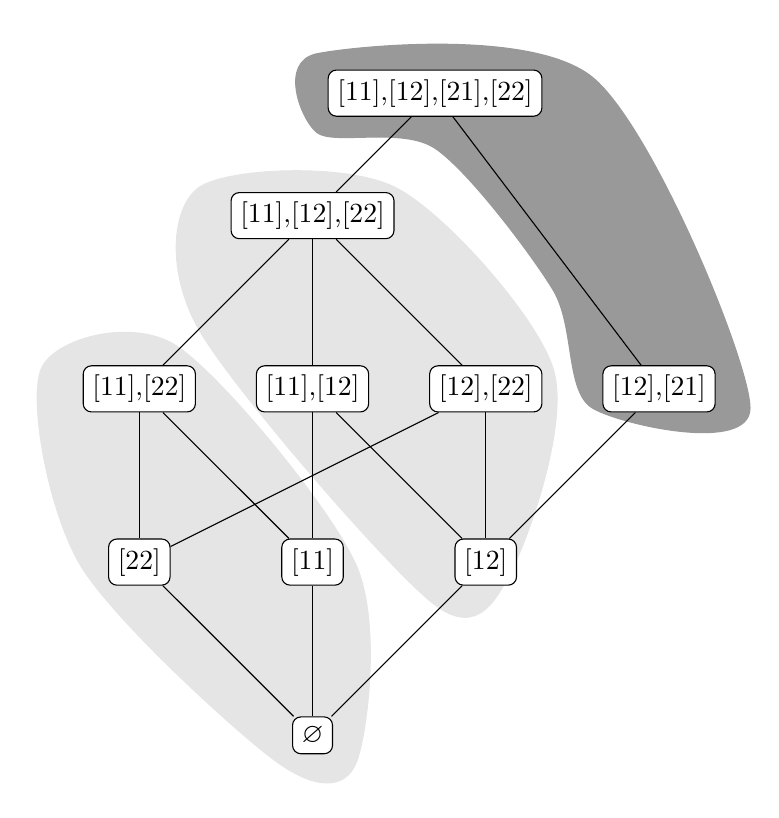
\begin{tikzpicture}
[align=center,node distance=2.2cm]
\tikzstyle{plain}=[fill=white,rounded corners=3pt, draw]

\draw node [plain] (1234) {[11],[12],[21],[22]};
\draw node [plain,below left of=1234] (124) {[11],[12],[22]};
\draw node [plain,below of=124] (12) {[11],[12]};
\draw node [plain,left of=12] (14) {[11],[22]};
\draw node [plain,right of=12] (24) {[12],[22]};
\draw node [plain,right of=24] (23) {[12],[21]};

\draw node [plain,below of=12] (1) {[11]};
\draw node [plain,left of=1] (4) {[22]};
\draw node [plain,right of=1] (2) {[12]};
\draw node [plain,below of=1] (empty) {$\varnothing$};

\draw  (1234) -- (124);
\draw (124) -- (12);
\draw (124) -- (24);
\draw (124) -- (14);
\draw  (1234) -- (23);
\path (23) edge (2);
\draw (1) -- (empty);
\draw (2) -- (empty);
\draw (4) -- (empty);
\draw (14) -- (4);
\draw (14) -- (1);
\draw (12) -- (2);
\draw (12) -- (1);
\draw (24) -- (4);
\draw (24) -- (2);
\begin{pgfonlayer}{background layer}
\filldraw [gray6] plot [smooth cycle] coordinates {(-1.5,-0.5)(-1.5,0.5)(2,0.2)(4,-4)(2,-4)(1.5,-2.5)(0,-0.7)};
\filldraw [gray9] plot [smooth cycle] coordinates {(-0.5,-1.2)(-3,-1.2)(-3,-3)(0,-6.5)(1,-6)(1.5,-3.5)};
\filldraw [gray9] plot [smooth cycle] coordinates {(-3.3,-3.2)(-5,-3.5)(-4.5,-6)(-2,-8.5)(-1,-8.5)(-1,-6)};


\end{pgfonlayer}

\end{tikzpicture}
\caption{The subsemigroup lattice of $\cT_2$, alternative classification. The singular part is indicated by the lowest light gray blob. The other light gray group is an identical copy of the singular part, just the identity adjoined to each subsemigroup. The dark grey part consists of the subsemigroups containing nontrivial permutations. The size of the dark group gets smaller relative to the singular part for higher degrees.}
\label{fig:T2subsAlt}
\end{figure}
$\cT_2$ has only four elements and consequently the search space size is only $2^4=16$.
It is an easy exercise to find all of its subsemigroups. 
Using one-line notation for transformations, we order the elements lexicographically, 1=[1,1], 2=[1,2], 3=[2,1], 4=[2,2]. Here are the closed subarrays.
\begin{tikzpicture}
[align=center,node distance=2.2cm]
\tikzstyle{plain}=[fill=white,rounded corners=3pt, draw]

\draw node [plain] (1234) {[11],[12],[21],[22]};
\draw node [plain,below left of=1234] (124) {[11],[12],[22]};
\draw node [plain,below of=124] (12) {[11],[12]};
\draw node [plain,left of=12] (14) {[11],[22]};
\draw node [plain,right of=12] (24) {[12],[22]};
\draw node [plain,right of=24] (23) {[12],[21]};

\draw node [plain,below of=12] (1) {[11]};
\draw node [plain,left of=1] (4) {[22]};
\draw node [plain,right of=1] (2) {[12]};
\draw node [plain,below of=1] (empty) {$\varnothing$};

\draw  (1234) -- (124);
\draw (124) -- (12);
\draw (124) -- (24);
\draw (124) -- (14);
\draw  (1234) -- (23);
\path (23) edge (2);
\draw (1) -- (empty);
\draw (2) -- (empty);
\draw (4) -- (empty);
\draw (14) -- (4);
\draw (14) -- (1);
\draw (12) -- (2);
\draw (12) -- (1);
\draw (24) -- (4);
\draw (24) -- (2);
\begin{pgfonlayer}{background layer}
\filldraw [dgr] plot [smooth cycle] coordinates {(1.5,-4.3)(-2.5,-4.2) (-2.3,-3.3) (1.5,-3.4)};
\filldraw [lgr] plot [smooth cycle] coordinates {(-4,-5.2) (2,-5.5) (1,-6.5)(-4.5,-6.6)};
\filldraw [dgr] plot [smooth cycle] coordinates {(-4,-5.5) (-1.2,-5.6) (-1.2,-6.3)(-4,-6.4)};
\end{pgfonlayer}

\end{tikzpicture}
Using these we can draw the subsemigroup lattice (Fig.\ \ref{fig:T2subs}).
It also shows that it is possible that isomorphic subsemigroups are not conjugate.

An obvious classification of $\Sub(\cT_2)$ can be done according to the sizes of the subsemigroups (Fig.\ \ref{fig:T2subs}).
It turns out that another way of partitioning the elements will also be important for higher degrees. 
One big chunk of the subsemigroup lattice of $\cT_n$ formed by the subsemigroups of the singular part, $\Sub(K_{n,n-1})$, and this has an order-isomorphic copy when we adjoin the identity of $\cT_n$ to each subsemigroup.
The remaining part is the set of subsemigroups that contain nontrivial permutations. 
Since we have no problems with fully calculating and displaying $\Sub(\cT_2)$, this division has no significance, but can be visualized easily (Fig.\ \ref{fig:T2subsAlt}).

\subsection{$\cT_3$, The Brute-force Doable}
The search space size for $\cT_3$ is $2^{3^3}=134217728$, approximately 134.2 million, thus exhaustive enumeration of subsets is still possible, though it takes many hours on a desktop computer.
In contrast, using the minimal extension method (Section \ref{sec:minext}) together with equivalent generators trick (Section \ref{sec:equivgen}) the calculation is seemingly instantaneous.
For generating the 283 conjugacy classes only 5362 subsets need to be checked. For all the 1299 subsemigroups 25041 checks are required. This demonstrated efficiency of the graph search algorithm makes our approach feasible.

\begin{table}[h]
\small
\renewcommand{\tabcolsep}{1pt}
\renewcommand{\arraystretch}{1}
\begin{tabular}{|c|c|c|c|c|c|c|c|c|c|c|c|c|c|c|c|c|c|c|c|c|c|c|c|c|c|c|c|c|}
\hline
Order&0&1&2&3& 4 & 5 & 6 & 7 & 8 & 9 & 10 & 11 & 12 & 13 & 14 & 15 & 16 & 17 & 18 & 19 & 20 & 21 & 22 & 23 & 24 & 25 & 26 & 27\\
\hline
\#conj&1& \cellcolor{gray9}3& \cellcolor{gray9}10& \cellcolor{gray9}19& \cellcolor{gray9}28& \cellcolor{gray9}38&42&38&30&25&14&12&7&3&1&3&2&2& & &  &1&1&1&1& &  &1\\
\hline
\#isom&1& \cellcolor{gray9}1& \cellcolor{gray9}5& \cellcolor{gray9}15& \cellcolor{gray9}24& \cellcolor{gray9}37&42&38&30&25&14&12&7&3&1&3&2&2& & &  &1&1&1&1& &  &1\\
\hline
\end{tabular}
\normalsize
\caption{The frequency distribution of conjugacy and isomorphism classes of $\Sub(\cT_3)$.}
\label{tab:T3freqs}
\end{table}
Classifying according to the sizes of the subsets is summarized in  Table \ref{tab:T3freqs}.
It is easy to see why there are no transformation semigroups on 3 points of size 25 and 26.
The biggest maximal subsemigroup is of order 24, so there is nothing in between that and $\cT_3$. On the other hand, we have no such explanation for orders 18,19 and 20. 

\begin{table}[h]
\small
\renewcommand{\tabcolsep}{1pt}
\renewcommand{\arraystretch}{1}
\begin{tabular}{|c|c|c|c|c|c|c|c|c|}
\hline
\#generators&0&1&2&3& 4 & 5 & 6 \\
\hline
\#conjugacy classes &1&  7& 46& 101& 85& 36& 7 \\
\hline
\end{tabular}
\normalsize
\caption{$n$-generatedness of conjugacy classes of $\Sub(\cT_3)$. The number of generators in a minimal size minimal generating set and the number of conjugacy classes with that many minimal generators.}
\label{tab:T3ngeneratedness}
\end{table}
We can also apply the minimal generating sets method (Section \ref{sec:mingen}), yielding Table \ref{tab:T3ngeneratedness}.

A semigroup $S$ is \emph{nilpotent} if $S^n=\{0\}$ for some $n\in\mathbb{N}$.
It is $k$-nilpotent if $k$ is the minimal such number.
 In other words, being $k$-nilpotent means that any product with at least $k$ elements yields the zero element.
Instead of calculating $S^k$ in total we can just take a random element $t$ and keep checking all $k$-tuples whether the result of the corresponding is $t$. The worst case is when $S$ is indeed $k$-nilpotent.

It turns out that that there are only 4 different nilpotent transformation semigroups on 3 points.
The trivial monoid is 1-nilpotent and it can be realized by three different ways: by the identity transformation, by a constant map, and by a conjugate of $[1,1,3]$.
The only $2$-nilpotent conjugacy class has the representative $\{[1,1,1],[1,1,3]\}$.

\subsection{$\cT_4$, The Parallel Possible }

The practical calculation of  $\Sub(\cT_4)$ is done by climbing up the ideal hierarchy.
We can jump over the first ideal.

\begin{enumerate}
\item Calculate $\Sub_{\cS_4}(K_{4,3}/K_{4,2})$ by the minimal extension algorithm (Section \ref{sec:minext}). There are 10 002 390, slightly more than 10 million conjugacy classes.  
\item \emph{In parallel}, enumerate all lower torsos for all the upper torsos derived from  $\Sub_{\cS_4}(K_{4,3}/K_{4,2})$ with the limited enumeration method (Section \ref{sec:lowertorso}). This gives $\Sub_{\cS_4}(K_{4,3})$, with  65 997 018 conjugacy classes. The calculation is truly parallel since the upper torsos always differ, so there is no need for merging the elements. By extending the empty upper torso we get $\Sub_{\cS_4}(K_{4,2})$.
\item To get the isomorphic copy of the singular part, we simplu adjoin the identity to all subsemigroups in $\Sub_{\cS_4}(K_{4,3})$. Call this set $C$.
Purely administrative step.
\item Calculate $\Sub_{\cS_4}(\cS_4)$ with minimal extensions. These are all closed upper torsos. This is a lot easier subgroup enumeration problem.
\item \emph{In parallel}, find all lower torsos for all nontrivial subgroups in $\Sub_{\cS_4}(\cS_4)$. This  is $P$, the set subsemigroups of $\cT_4$ with nontrivial permutations, including the subgroups as well. This part corresponds to the dark blob on Figure \ref{fig:T2subsAlt}.
Though the search space is the set of subsets of $K_{4,3}$, the search is surprisingly quick.
This is due to the fact that a subgroup acts on the singular part, making each minimal extension into a huge step.
For instance, there are only 71 146 lower torsos in $K_{4,3}$ for $\mathbb{Z}_2$.
\item $\Sub(\cT_4)=\Sub(K_{4,3})\cup C \cup P$. The set of subsemigroups of the ideal part, its copy with the identity adjoined to each subsemigroup, and the subsemigroups with permutations.
\end{enumerate}

\begin{table}
\renewcommand{\tabcolsep}{2pt}
\renewcommand{\arraystretch}{1}
\begin{tabular}{|c|r|r|r||r|r|r||r|r|r|}
\hline
$K_{i,j}$ & \multicolumn{3}{c||}{$j=1$} & \multicolumn{3}{c||}{2} & \multicolumn{3}{c|}{3} \\
\hline
$i=2$ & 4&3&3   & \cellcolor{gray9}  & \cellcolor{gray9}&  \cellcolor{gray9} & \cellcolor{gray9}  &\cellcolor{gray9} &\cellcolor{gray9}\\
\hline
$3$ &  8&4&4  &  600 & 123 & 118  & \cellcolor{gray9}  & \cellcolor{gray9}&\cellcolor{gray9}\\
\hline
$4$ & 16&5&5  &  3 788 252 & 162 332 & 151 959  & 1 580 548 624  & 65 997 018&TBA\\
\hline
$n$ & $2^n$&$n+1$&$n+1$    &    & &    &    & & \\
\hline

\end{tabular}
\caption{Number of subsemigroups of ideals in of full transformation semigroups. The second and third numbers are the number of distinct subsemigroups up to conjugacy and isomorphism.}
\end{table}



\begin{figure}
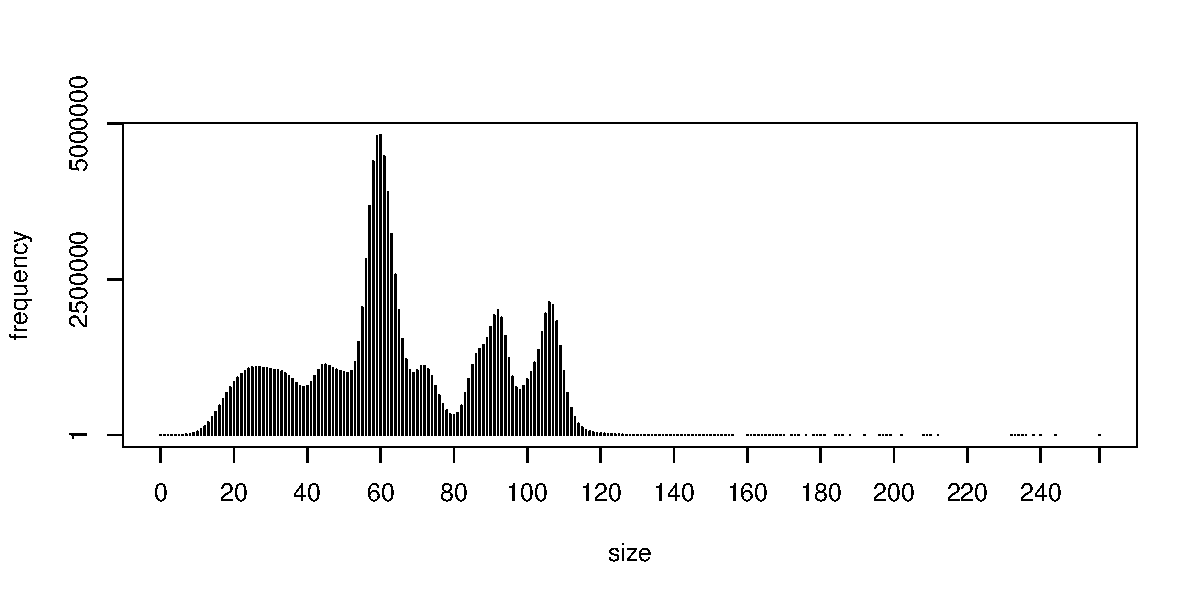
\includegraphics[width=\textwidth]{SubT4distrib}
\caption{The size distribution of $\Sub_{\cS_4}(\cT_4)$. The maximum is at size 60. There are 58 different size values with no subsemigroup (no corresponding dot in the figure).}
%\caption{The size distribution of of $\Sub(\cT_4)$. No line/dot is drawn where the value is 0.}
\label{fig:SubT4SizeDistrib}
\end{figure}
The size distribution of $\Sub(\cT_4)$ shows an interesting pattern (Fig.\ \ref{fig:SubT4SizeDistrib}).
For subgroups of a group only the divisors of its order have nonzero frequency values.
For all subsets the maximal binomial coefficient defines the peak value.
For $\Sub(\cT_4)$ the situation is more involved.
The numbers are big and they make the impression of continuous change with several peaks.
To explain the shape of the  distribution a systematic study of the size classes is needed. 

There are only 22 nonempty nilpotent subsemigroups of $\cT_4$ up to isomorphism, 4 of them are 1-nilpotent, 7 are 2-nilpotent and 11 are 3-nilpotent.
The biggest 3-nilpotent subsemigroup has 6 elements:
$$\left\{[1,1,1,1],[1,1,1,2],[1,1,1,3],[1,1,2,1],[1,1,2,2],[1,1,2,3]\right\}.$$
It is an interesting question whether the pattern seen here is a general recipe for constructing maximal 3-nilpotent transformation semigroups.
\section{Summary and Conclusion}
We enumerated and classified all transformation semigroups up to degree 4.
It turns out while enumerating abstract semigroups yields mostly 3-nilpotent semigroups, enumerating transformation semigroups gives asymptotically vanishing amount of 3-nilpotent ones.

The methods developed here, with more concentrated effort and computational power,  may be able to partially enumerate $\Sub(\cT_5)$.
The closure algorithms in Section \ref{sec:multab} need full complexity analysis before attacking the next degree. 

However, a better usage of the results would be to investigate the possibility of a more constructive theory of all transformation semigroups.
For instance, by studying how many different ways $\Sub(\cT_n)$ is embedded into $\Sub(\cT_{n+1})$, we can probably estimate $|\Sub(\cT_{n+1})|$, or even construct some recursive formula.
\begin{table}
\renewcommand{\arraystretch}{1}
\begin{tabular}{|c|r|r|r|}
\hline
 & \#subsemigroups & \#conjugacy classes & \#isomorphism classes \\
\hline
$\cT_0$ & 1  & 1 (1)& 1\\
\hline
$\cT_1$ & 2  & 2 (2)& 2\\
\hline
$\cT_2$ & 10  & 8 (3)& 7\\
\hline
$\cT_3$ & 1 299 & 283 (5)& 267\\
\hline
$\cT_4$ & 3 161 965 550 & 132 069 776 (23)& TBA\\
\hline
\end{tabular}
\caption{Number of subsemigroups of full transformation semigroups. Values in parantheses are the number of nilpotent classes.}
\end{table}


\bibliography{subsemi}
\bibliographystyle{plain}

\end{document}